\section{/home/aakash/mlpack/src/mlpack/core/tree/octree.hpp File Reference}
\label{octree_8hpp}\index{/home/aakash/mlpack/src/mlpack/core/tree/octree.\+hpp@{/home/aakash/mlpack/src/mlpack/core/tree/octree.\+hpp}}
Include dependency graph for octree.\+hpp\+:
\nopagebreak
\begin{figure}[H]
\begin{center}
\leavevmode
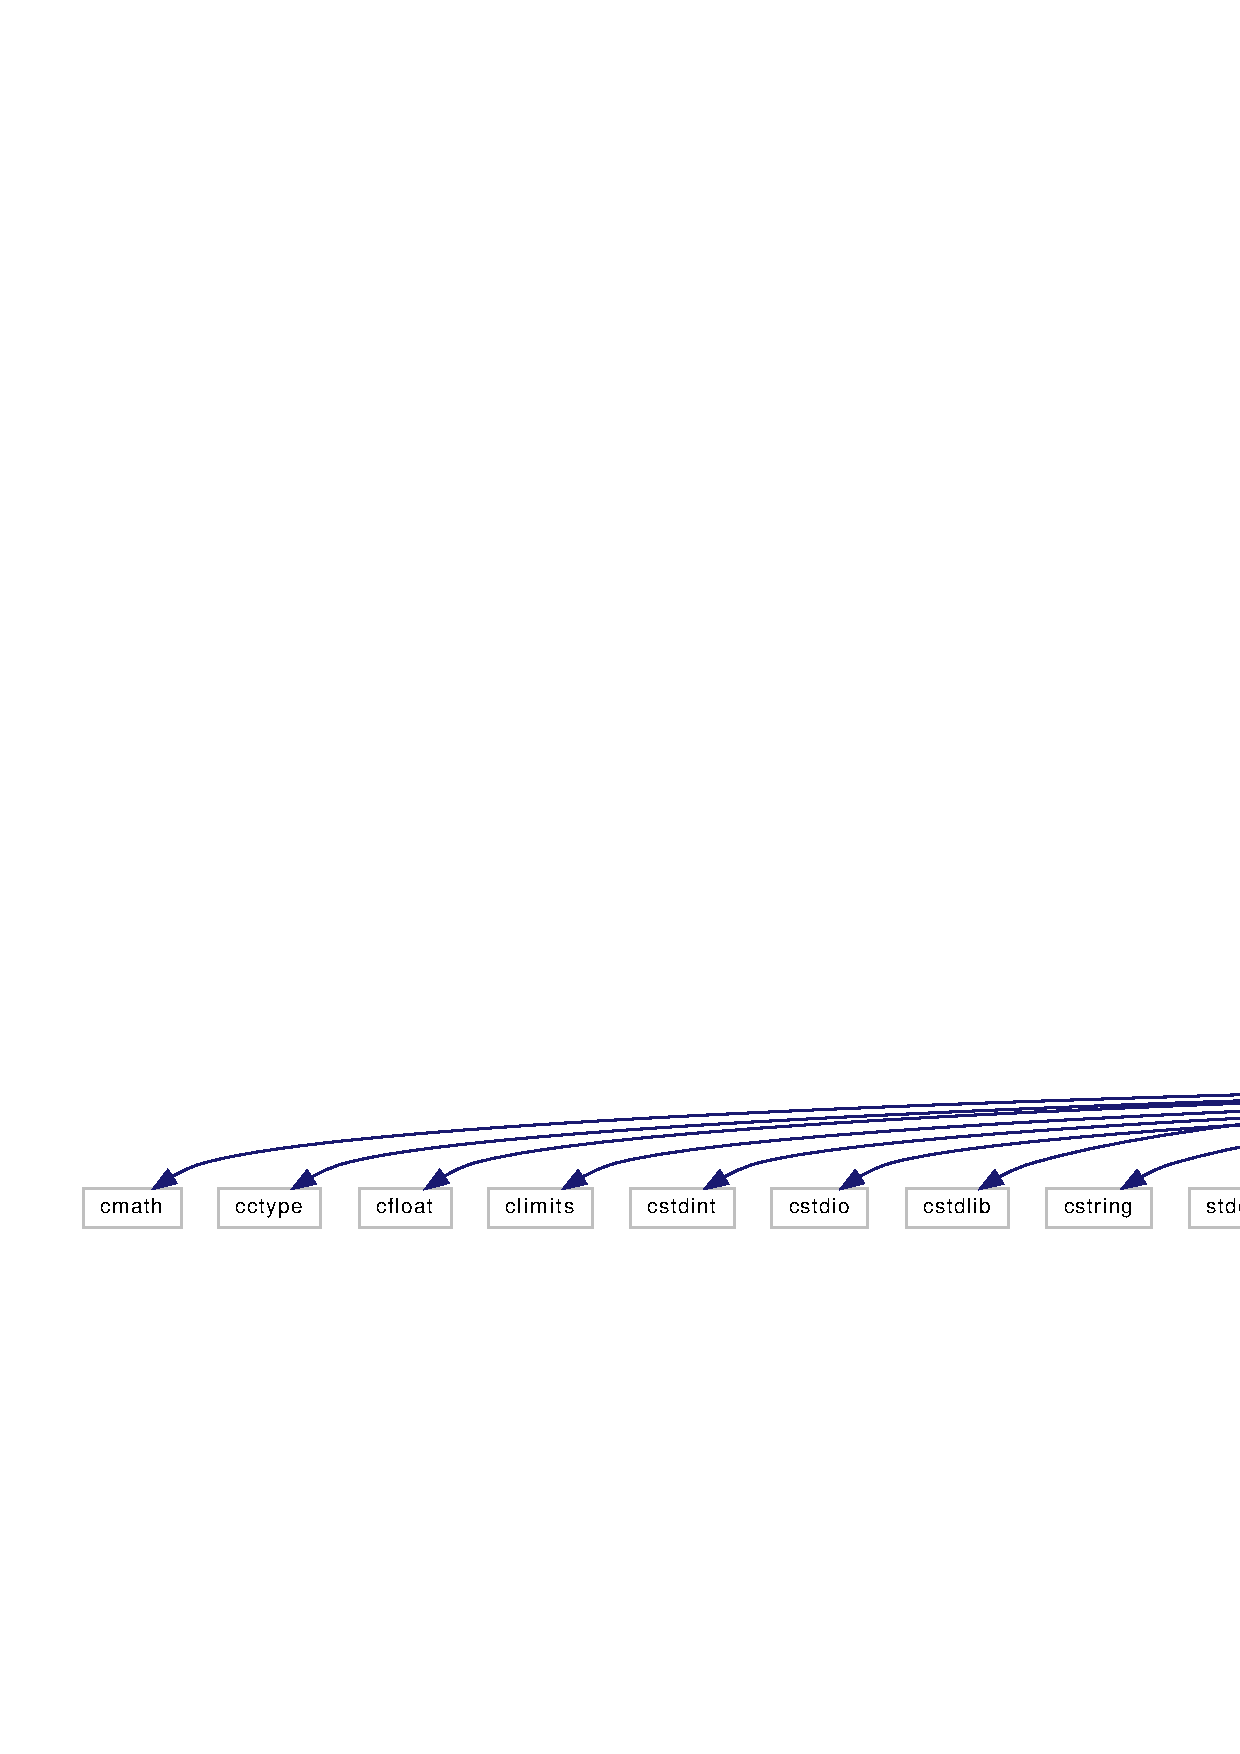
\includegraphics[width=350pt]{octree_8hpp__incl}
\end{center}
\end{figure}
This graph shows which files directly or indirectly include this file\+:
\nopagebreak
\begin{figure}[H]
\begin{center}
\leavevmode
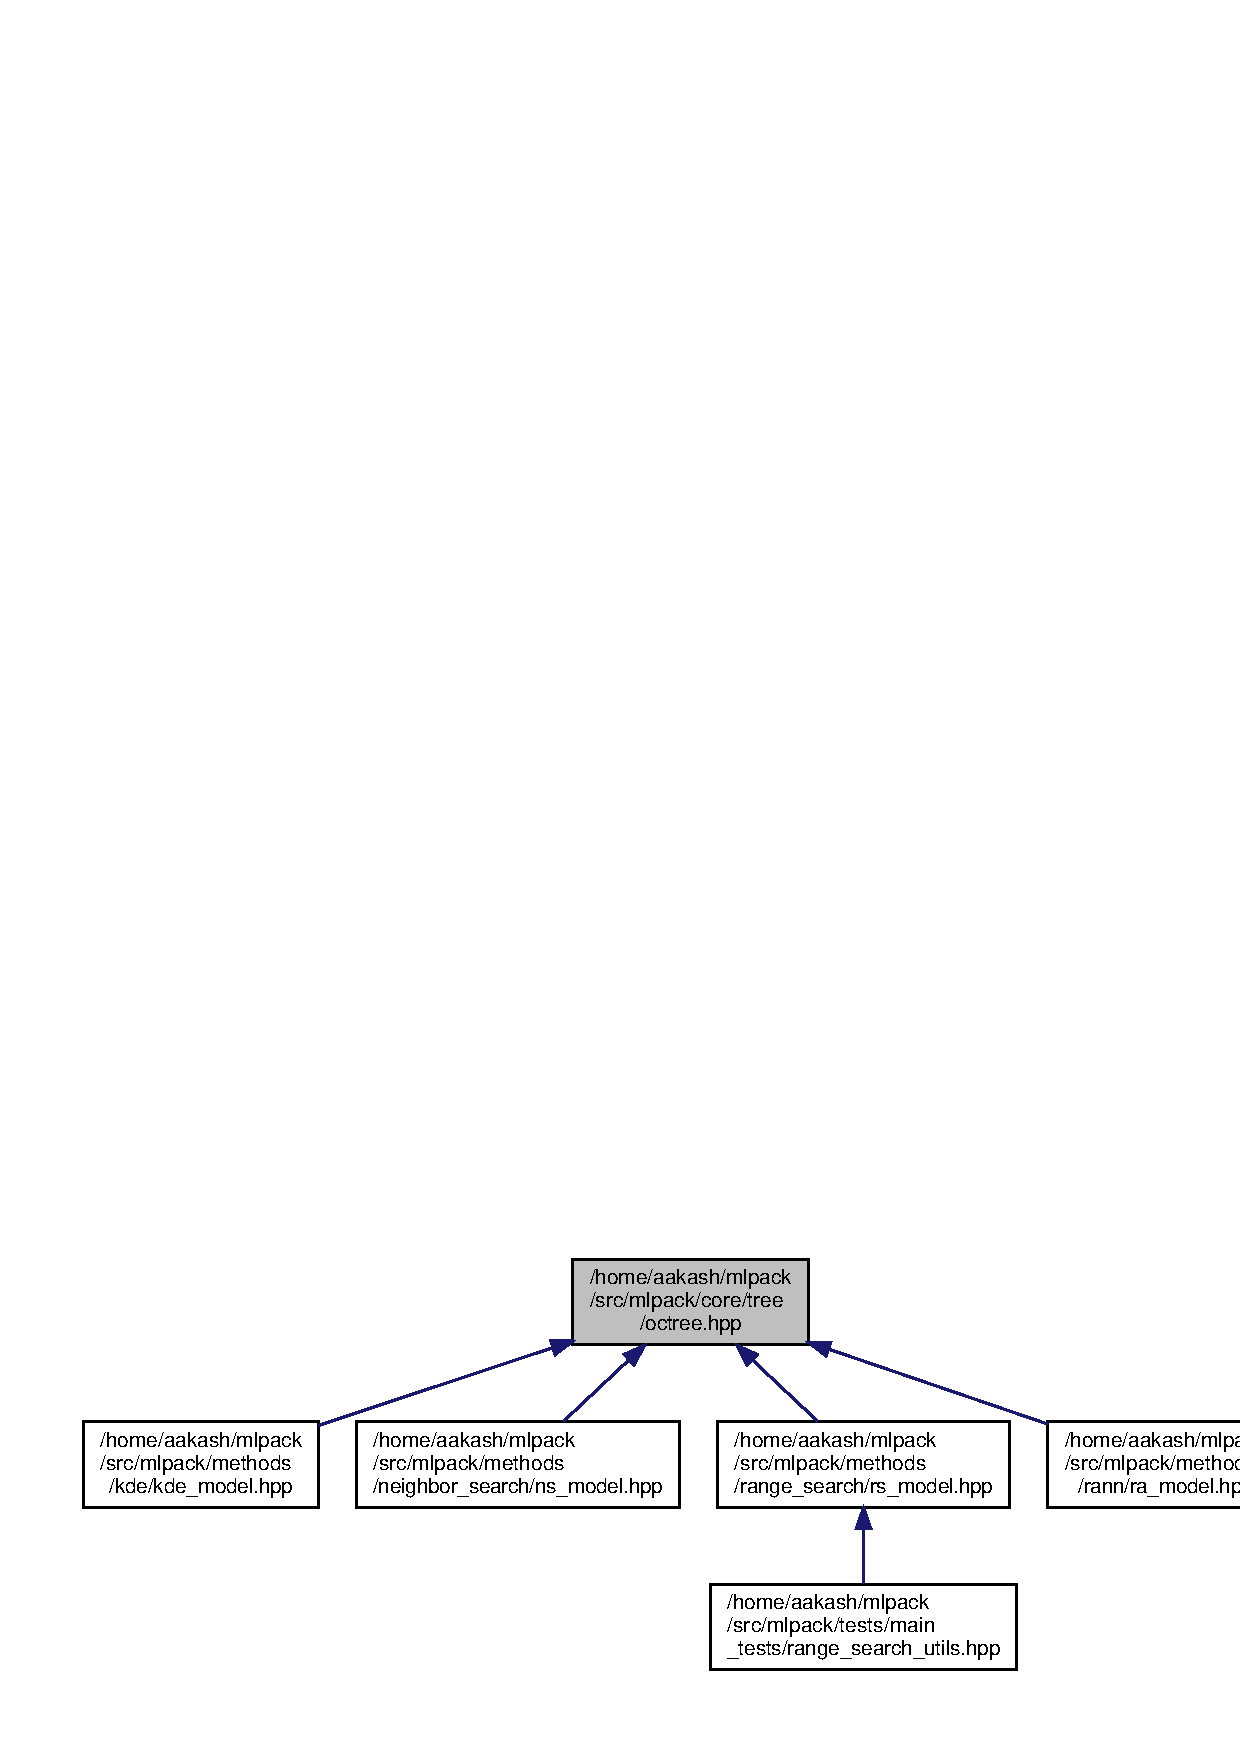
\includegraphics[width=350pt]{octree_8hpp__dep__incl}
\end{center}
\end{figure}


\subsection{Detailed Description}
\begin{DoxyAuthor}{Author}
Ryan Curtin
\end{DoxyAuthor}
Include all the necessary files to use the Octree class.

mlpack is free software; you may redistribute it and/or modify it under the terms of the 3-\/clause B\+SD license. You should have received a copy of the 3-\/clause B\+SD license along with mlpack. If not, see {\tt http\+://www.\+opensource.\+org/licenses/\+B\+S\+D-\/3-\/\+Clause} for more information. 